\chapter{Pure Functional Time-Driven ABS}
\label{ch:timedriven}

In this chapter, we pose solutions to the previously mentioned problems by derive a pure functional approach for time-driven ABS through the example of the agent-based SIR model. We start out with a first approach in Yampa and show its limitations. Then we generalise it to a more powerful approach, which utilises Monadic Stream Functions (MSF), a generalisation of FRP. Finally we add a structured environment, making the example more interesting and showing the real strength of ABS over other simulation methodologies like System Dynamics and Discrete Event Simulation \footnote{The code of all steps can be accessed freely through the following URL: \url{https://github.com/thalerjonathan/phd/tree/master/public/purefunctionalepidemics/code}}.

\section{Case Study I: SIR}
\label{sec:concurrent_sir}
Our first case study is the SIR model as introduced in Chapter \ref{sec:sir_model}. The aim of this case study is to investigate the potential speed up a concurrent \textit{STM} implementation gains over a sequential one under varying number of CPU cores and agents. The behaviour of the agents is quite simple and the interactions are happening indirectly through the environment, where reads from the environment outnumber the writes to it by far. Further, a comparison to a lock-based implementation with the \textit{IO} Monad is done to understand that \textit{STM} is also able to outperform traditional concurrency, \textit{in a pure functional ABS setting} while still retaining its greater static guarantees than \textit{IO} \footnote{The code of all three implementations is available at \url{https://github.com/thalerjonathan/phd/tree/master/public/stmabs/code/SIR}}.

\begin{enumerate}
	\item Sequential - this is the original implementation as discussed in Chapter \ref{sec:adding_env}, where the discrete 2D environment is shared amongst all agents as read-only data and the agents are executed sequentially within the main thread without any concurrency.
	\item STM - this is the same implementation as the \textit{Sequential} one but agents run now in the \textit{STM} Monad and have access to the discrete 2D environment through a transactional variable \textit{TVar}. This means that the agents now communicate indirectly by reads and writes through the \textit{TVar}.
	\item Lock-Based - this follows the \textit{STM} implementation, with the agents running in \textit{IO}. They share the discrete 2D environment using an \textit{IORef} and have access to an \textit{MVar} lock to synchronise access to it.
\end{enumerate}

Each experiment was run until $t = 100$ and stepped using $\Delta t = 0.1$. For each experiment we conducted 8 runs on our machine (see Table \ref{tab:machine_specs}) under no additional work-load and report the mean. %Further, we checked the visual outputs and the dynamics and they look qualitatively the same as the reference \textit{Sequential}. We could have used more rigour and properly validated the implementations against the formal specification using tests as we do in Chapter Property-based testing but we leave this for further res.
In the experiments we varied the number of agents (grid size) as well as the number of cores when running concurrently - the numbers are always indicated clearly.

\begin{table}
	\centering
	\begin{tabular}{ c || c }
		OS & Fedora 28, 64-bit \\ \hline
		RAM & 16 GByte \\ \hline
		CPU & Intel i5-4670K @ 3.4GHz \\ \hline
		HD & 250Gbyte SSD \\ \hline
		Haskell & GHC 8.2.2
	\end{tabular}
	
	\caption{Machine and Software specs for all experiments}
	\label{tab:machine_specs}
\end{table}

\subsection{Constant Grid Size, Varying Cores}
In this experiment we held the grid size constant to 51 x 51 (2,601 agents) and varied the cores. The results are reported in Table \ref{tab:constgrid_varyingcores}.

\begin{table}
	\centering
	\begin{tabular}{cc|c}
		\multicolumn{1}{ c||  }{\multirow{2}{*}{} } &
		\multicolumn{1}{ |c| }{Cores} & Duration      \\ \hline \hline 
		
		\multicolumn{1}{ c||  }{\multirow{1}{*}{Sequential} } &
		\multicolumn{1}{ |c| }{1} & 72.5      \\ \hline \hline 
		
		\multicolumn{1}{ c||  }{\multirow{4}{*}{Lock-Based} } &
		\multicolumn{1}{ |c| }{1} & 60.6       \\ \cline{2-3}
		\multicolumn{1}{ c||  }{}                       &
		\multicolumn{1}{ |c| }{2} & 42.8    \\ \cline{2-3}
		\multicolumn{1}{ c||  }{}                       &
		\multicolumn{1}{ |c| }{3} & 38.6    \\ \cline{2-3}
		\multicolumn{1}{ c||  }{}                       &
		\multicolumn{1}{ |c| }{4} & 41.6    \\ \hline \hline 
		
		\multicolumn{1}{ c||  }{\multirow{4}{*}{STM} } &
		\multicolumn{1}{ |c| }{1} & 53.2       \\ \cline{2-3}
		\multicolumn{1}{ c||  }{}                       &
		\multicolumn{1}{ |c| }{2} & 27.8    \\ \cline{2-3}
		\multicolumn{1}{ c||  }{}                       &
		\multicolumn{1}{ |c| }{3} & 21.8    \\ \cline{2-3}
		\multicolumn{1}{ c||  }{}                       &
		\multicolumn{1}{ |c| }{4} & \textbf{20.8}    \\ \hline \hline 
	\end{tabular}
  	
  	\caption{Experiments on 51x51 (2,601 agents) grid with varying number of cores. Timings in seconds (lower is better).}
	\label{tab:constgrid_varyingcores}
\end{table}

The \textit{STM} implementation running on 4 cores shows a speed up factor of 3.6 over \textit{Sequential}, which is a quite impressive number when considering that we can achieve at most a factor of 4 when running on 4 cores. It seems that \textit{STM} allow us to push the practical limit very close to the theoretical one, whereas the \textit{Lock-Based} approach just arrives at a factor of 1.74 on 4 cores.

Comparing the performance and scaling to multiple cores shows that the \textit{STM} implementation significantly outperforms the \textit{Lock-Based} one and scales better to multiple cores. The \textit{Lock-Based} implementation performs best with 3 cores and shows slightly worse performance on 4 cores as can be seen in Figure \ref{fig:core_duration_stm_io}. This is no surprise because the more cores are running at the same time, the more contention for the lock, thus the more likely synchronisation happening, resulting in higher potential for reduced performance. This is not an issue in \textit{STM} because no locks are taken in advance. 

\begin{figure}
	\centering
	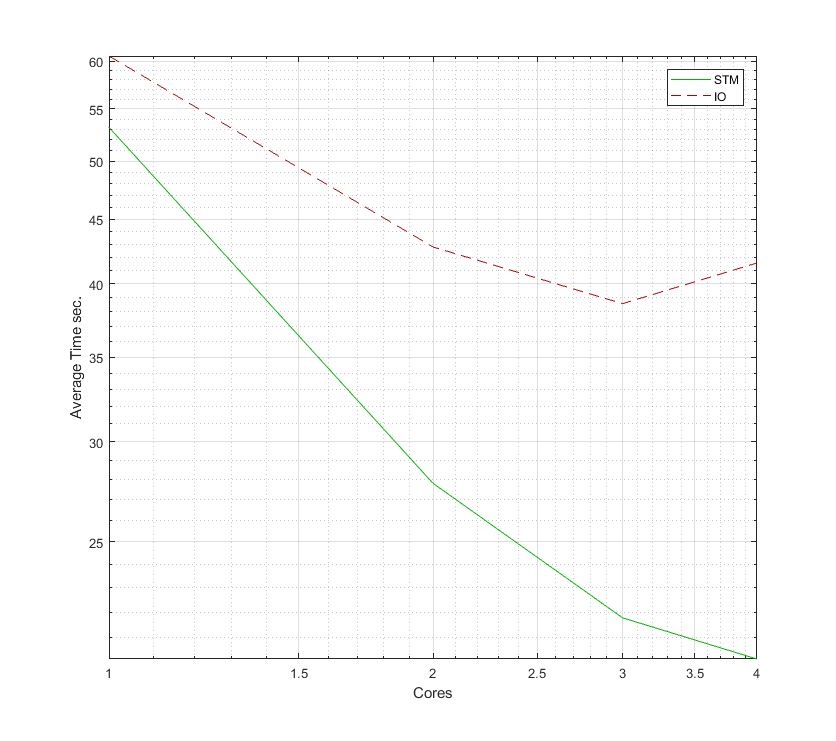
\includegraphics[width=0.8\textwidth, angle=0]{./fig/concurrentabs/sir/core_duration_stm_io.png}
	\caption{Comparison of performance and scaling on multiple cores of STM and Lock-Based. Note that the Lock-Based implementation seems to perform slightly worse on 4 than on 3 cores probably due to lock-contention.}
	\label{fig:core_duration_stm_io}
\end{figure}

\subsection{Varying Grid Size, Constant Cores}
In this experiment we varied the grid size and used always 4 cores. The results are reported in Table \ref{tab:varyinggrid_constcores} and plotted in Figure \ref{fig:varyinggrid_constcores}.

\begin{table}
	\centering
  	\begin{tabular}{ c || c | c | c }
        Grid-Size          & STM              & Lock-Based   & Ratio \\ \hline \hline 
   		51 x 51 (2,601)    & \textbf{20.2}    & 41.9         & 2.1 \\ \hline
   		101 x 101 (10,201) & \textbf{74.5}    & 170.5        & 2.3 \\ \hline
   		151 x 151 (22,801) & \textbf{168.5}   & 376.9        & 2.2 \\ \hline
   		201 x 201 (40,401) & \textbf{302.4}   & 672.0        & 2.2 \\ \hline
   		251 x 251 (63,001) & \textbf{495.7}   & 1,027.3      & 2.1 \\ \hline \hline
  	\end{tabular}

  	\caption{Performance on varying grid sizes. Timings in seconds (lower is better). Ratio compares STM to Lock-Based.}
	\label{tab:varyinggrid_constcores}
\end{table}

It is clear that the \textit{STM} implementation outperforms the \textit{Lock-Based} implementation by a substantial factor.

\begin{figure}
	\centering
	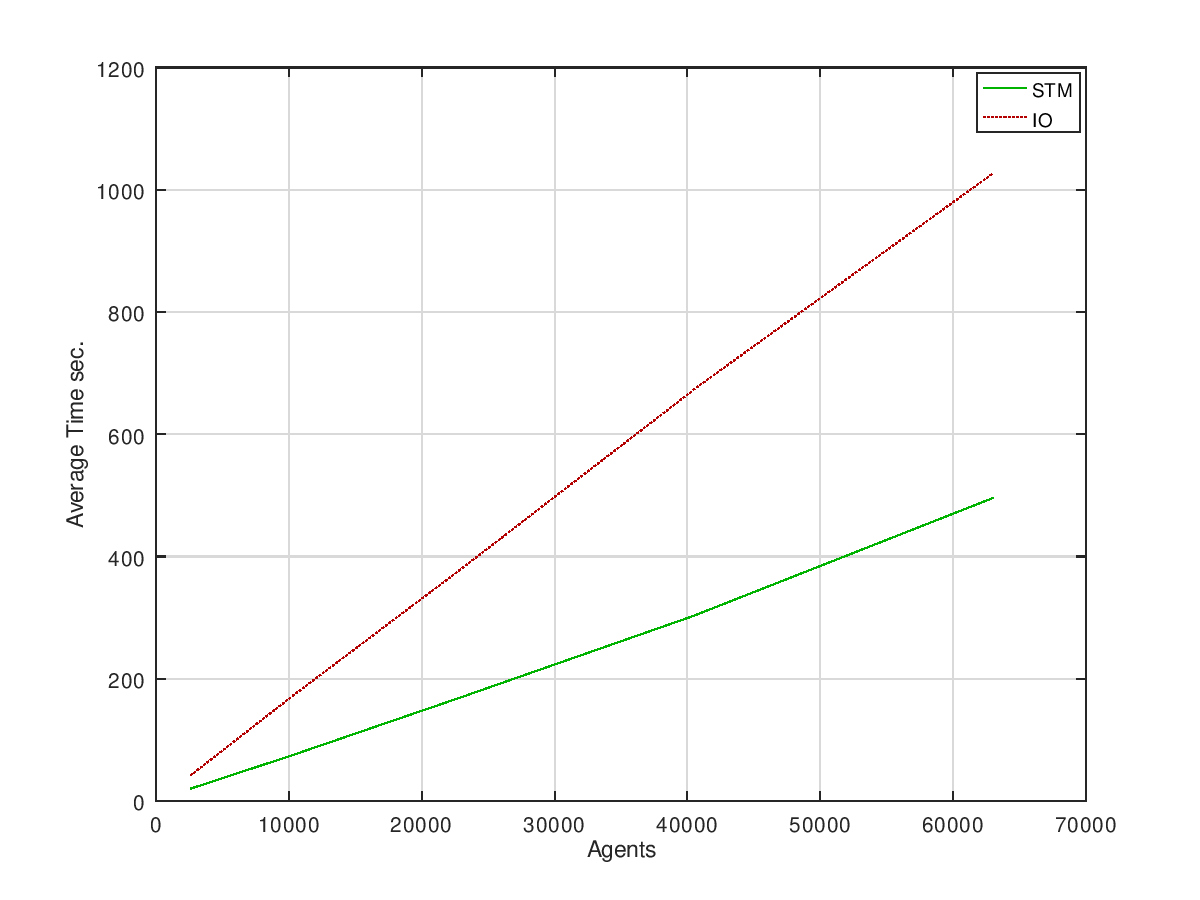
\includegraphics[width=1\textwidth, angle=0]{./fig/concurrentabs/sir/stm_io_varyinggrid_performance.png}
	\caption{Performance on varying grid sizes.}
	\label{fig:varyinggrid_constcores}
\end{figure}

\subsection{Retries}
Of very much interest when using STM is the retry-ratio, which obviously depends highly on the read-write patterns of the respective model. We used the \textit{stm-stats} library to record statistics of commits, retries and the ratio. The results are reported in Table \ref{tab:retries_stm}.

\begin{table}
	\centering
  	\begin{tabular}{ c || c | c | c }
        Grid-Size 		   & Commits    & Retries & Ratio \\ \hline \hline 
   		51 x 51 (2,601)    & 2,601,000  & 1306.5  & 0.0 \\ \hline
   		101 x 101 (10,201) & 10,201,000 & 3712.5  & 0.0 \\ \hline
   		151 x 151 (22,801) & 22,801,000 & 8189.5  & 0.0 \\ \hline
   		201 x 201 (40,401) & 40,401,000 & 13285.0 & 0.0 \\ \hline 
   		251 x 251 (63,001) & 63,001,000 & 21217.0 & 0.0 \\ \hline \hline
  	\end{tabular}
  	
  	\caption{Retry ratios on varying grid sizes on 4 cores.}
	\label{tab:retries_stm}
\end{table}

Independent of the number of agents we always have a retry-ratio of 0.0. This indicates that this model is \textit{very} well suited to STM, which is also directly reflected in the much better performance over the \textit{Lock-Based} implementation. Obviously this ratio stems from the fact that in our implementation we have \textit{very} few writes, which happen only in case when an agent changes from Susceptible to Infected or from Infected to Recovered. On the other hand, there are a very large number of reads due to indirect agent interaction. For \textit{STM} this is no problem because no lock is taken but the \textit{Lock-Based} approach is forced to conservatively take the lock to ensure mutual exclusive access to the critical section across all agents.

\subsection{Going Large-Scale}
To test how far we can scale up the number of cores in both the \textit{Lock-Based} and \textit{STM} cases, we ran two experiments, 51x51 and 251x251, on Amazon EC2 instances with a larger number of cores than our local machinery, starting with 16 and 32 to see if we are running into decreasing returns. The results are reported in Table \ref{tab:sir_varying_cores_amazon}.

\begin{table}
	\centering
  	\begin{tabular}{cc|c|c}
		\multicolumn{1}{ c||  }{\multirow{2}{*}{} } &
		\multicolumn{1}{ |c| }{Cores} & 51x51    & 251x251       \\ \hline \hline 
		
		\multicolumn{1}{ c||  }{\multirow{2}{*}{Lock-Based} } &
		\multicolumn{1}{ |c| }{16} & 72.5    & 1830.5       \\ \cline{2-4}
		\multicolumn{1}{ c||  }{}                       &
		\multicolumn{1}{ |c| }{32} & 73.1    & 1882.2      \\ \hline \hline 
		
		\multicolumn{1}{ c||  }{\multirow{2}{*}{STM} } &
		\multicolumn{1}{ |c| }{16} & \textbf{8.6}     & \textbf{237.0}       \\ \cline{2-4}
		\multicolumn{1}{ c||  }{}                       &
		\multicolumn{1}{ |c| }{32} & 12.0    & 248.7      \\ \hline \hline 
	\end{tabular}

  	\caption{Performance on varying cores on Amazon S2 Services. Timings in seconds (lower is better).}
	\label{tab:sir_varying_cores_amazon}
\end{table}

As expected, the \textit{Lock-Based} approach doesn't scale up to many cores because each additional core brings more contention to the lock, resulting in an even more decreased performance, even worse than the \textit{Sequential} implementation. This is particularly obvious in the 251x251 experiment because of the much larger number of concurrent agents. The \textit{STM} approach returns better performance on 16 cores but fails to scale further up to 32 where the performance drops below the one with 16 cores. In both STM cases we measured a retry-ratio of 0, thus we assume that with 32 cores we become limited by the overhead of STM transactions \cite{perfumo_limits_2008} because the workload of an STM action in our SIR implementation is quite small.

Compared to the \textit{Sequential} implementation, \textit{STM} reaches a speed up factor of 8.4 on 16 cores, which is still impressive but is much further away from the theoretical limit than in the case of only 4 cores -  a further indication that this model in particular and our approach in general does not scale up arbitrarily.

% NOTE: 0 retries in both cases means that the STM transactions themselves are becoming the bottleneck. this makes sens because the STM trasnactions in our SIR implementation are very small (especially recovered and infected agent) and could therefore really cause substantial overhead as pointed out by \cite{perfumo_limits_2008}
%16 cores 251x251: 0.0 retry-ratio
%32 cores 251x251: 0.0 retry ratio
%
%16 cores 51x51: 0.0 retry-ratio
%32 cores 51x51: 0.0 retry ratio

\subsection{Discussion}
The timing measurements speak a clear language: running in \textit{STM} and sharing state using a transactional variable \textit{TVar} is much more time-efficient than both the \textit{Sequential} and \textit{Lock-Based} approach. On 4 cores \textit{STM} achieves a speed up factor of 3.6, nearly reaching the theoretical limit.
Obviously both \textit{STM} and \textit{Lock-Based} sacrifices determinism: repeated runs might not lead to same dynamics despite same initial conditions. Still, by sticking to \textit{STM}, we get the guarantee that the source of this non-determinism is concurrency within the \textit{STM} monad but \textit{nothing else}. This we can not guarantee in the case of the \textit{Lock-Based} approach as all bets are off when running within \textit{IO}. The fact to have \textit{both} the better performance \textit{and} the stronger static guarantees in the \textit{STM} approach makes it \textit{very} compelling.

\section{First step: pure computation}
\label{sec:timedriven_firststep}
As described in Chapter \ref{sec:back_frp}, Arrowized FRP \cite{hughes_generalising_2000} is a way to implement systems with continuous and discrete time-semantics, where the central concept is the signal function, which can be understood as a process over time, mapping an input- to an output-signal. Technically speaking, a signal function is a continuation which allows to capture state using closures and hides away the $\Delta t$. This has the effect, that the $\Delta t$ is never exposed explicitly to the programmer, meaning the programmer can neither manipulate it nor define non-causal systems where a signal function depends on a signal in the future. Early, non-arrowized implementations of FRP had this flaw and it was only possible through arrowized FRP to solve this issue, as arrows parametrise also over the input-type, thus making it possible to deal with this issue.

As already pointed out, agents need to perceive time, which means that the concept of processes over time is an ideal match for our agents and our system as a whole, thus we will implement them and the whole system as signal functions.

According to the model, every agent makes \textit{on average} contact with $\beta$ random other agents per time unit. In ABS we can only contact discrete agents, thus we model this by generating a random event on average every $\frac{1}{\beta}$ time units. We need to sample from an exponential distribution because the rate is proportional to the size of the population \cite{borshchev_system_2004}. Note that an agent does not know the other agents' state when making contact with it, thus we need a mechanism in which agents reveal their state in which they are in \textit{at the moment of making contact}. This mechanism is an implementation detail, which we will derive in our implementation steps. For now we only assume that agents can make contact with each other somehow.

The \textit{parallel} strategy matches the semantics of the agent-based SIR model due to the underlying roots in the System Dynamics approach. As discussed already in Chapter \ref{sub:par_strategy}, in the parallel update-strategy, the agents act conceptually all at the same time in lock-step. This implies that they observe the same system state during a time-step and actions of an agent are only visible in the next time-step - they are isolated from each other. As will become apparent, FP can be used to enforce the correct application of this strategy through the strong static type-system, at compile-time.

We start by defining the SIR states as Algebraic Data Type (ADT) and our agents as signal functions (SF), which receive the SIR states of all agents form the previous step as input and outputs the current SIR state of the agent. This definition, and the fact that Yampa is not monadic, guarantees already at compile, that the agents are isolated from each other, enforcing the \textit{parallel} lock-step semantics of the model.

\begin{HaskellCode}
data SIRState = Susceptible | Infected | Recovered

type SIRAgent = SF [SIRState] SIRState 

sirAgent :: RandomGen g => g -> SIRState -> SIRAgent
sirAgent g Susceptible = susceptibleAgent g
sirAgent g Infected    = infectedAgent g
sirAgent _ Recovered   = recoveredAgent
\end{HaskellCode}

Depending on the initial state we return the corresponding behaviour. Note that we are passing a random-number generator instead of running in the \textit{Rand} Monad because signal functions as implemented in Yampa are not capable of being monadic. 

We see that the recovered agent ignores the random-number generator because a recovered agent does nothing, stays immune forever and can not get infected again in this model. Thus a recovered agent is a consuming state from which there is no escape, it simply acts as a sink, constantly returning \textit{Recovered}:

\begin{HaskellCode}
recoveredAgent :: SIRAgent
recoveredAgent = arr (const Recovered)
\end{HaskellCode}

Next, we implement the behaviour of a susceptible agent. It makes contact \textit{on average} with $\beta$ other random agents. For every \textit{infected} agent it gets into contact with, it becomes infected with a probability of $\gamma$. If an infection happens, it makes the transition to the \textit{Infected} state. To make contact, it gets fed the states of all agents in the system from the previous time-step, so it can draw random contacts. Observing the states of all agents from the previous step allows for a very simple, one-directional form of making contact between agents. Although simple, it works perfectly for this approach in particular and for time-driven ABS in general. We will discuss a more complex interaction mechanism between agents in the next Chapter \ref{ch:eventdriven} on event-driven ABS.

A susceptible agent behaves as susceptible until it becomes infected. Upon infection an \textit{Event} is returned, which results in switching into the \textit{infectedAgent} SF, which causes the agent to behave as an infected agent from that moment on. When an infection event occurs we change the behaviour of an agent using the Yampa combinator \textit{switch}, which is quite elegant and expressive as it makes the change of behaviour at the occurrence of an event explicit. Note that to make contact \textit{on average}, we use Yampas \textit{occasionally} function which requires us to carefully select the right $\Delta t$ for sampling the system as will be shown in results. 

Note the use of \textit{iPre :: a $\rightarrow$ SF a a}, which delays the input signal by one sample, taking an initial value for the output at time zero. The reason for it is that we need to delay the transition from susceptible to infected by one step due to the semantics of the \textit{switch} combinator: whenever the switching event occurs, the signal function into which is switched will be run at the time of the event occurrence. This means that a susceptible agent could make a transition to recovered within one time-step, which we want to prevent, because the semantics should be that only one state-transition can happen per time-step.

\begin{HaskellCode}
susceptibleAgent :: RandomGen g => g -> SIRAgent
susceptibleAgent g 
    = switch 
      -- delay switching by 1 step to prevent against transition
      -- from Susceptible to Recovered within one time-step
      (susceptible g >>> iPre (Susceptible, NoEvent)) 
      (const (infectedAgent g))
  where
    susceptible :: RandomGen g => g -> SF [SIRState] (SIRState, Event ())
    susceptible g = proc as -> do
      -- generate make contact events with given rate
      makeContact <- occasionally g (1 / contactRate) () -< ()
      if isEvent makeContact
        then (do
          -- draw random element from the list
          a <- drawRandomElemSF g -< as
          case a of
            Infected -> do
              -- returns True with given probability
              i <- randomBoolSF g infectivity -< ()
              if i
                -- got infected, signal to switch through Event
                then returnA -< (Infected, Event ())
                else returnA -< (Susceptible, NoEvent)
             _       -> returnA -< (Susceptible, NoEvent))
        else returnA -< (Susceptible, NoEvent)
\end{HaskellCode}

To deal with randomness in an FRP way, we implemented additional signal functions built on the \textit{noiseR} function provided by Yampa. This is an example for the stream character and statefulness of a signal function as it allows to keep track of the changed random-number generator internally through the use of continuations and closures. Here we provide the implementation of \textit{randomBoolSF}, \textit{drawRandomElemSF} works similar but takes a list as input and returns a randomly chosen element from it:

\begin{HaskellCode}
randomBoolSF :: RandomGen g => g -> Double -> SF () Bool
randomBoolSF g p = proc _ -> do
  r <- noiseR ((0, 1) :: (Double, Double)) g -< ()
  returnA -< (r <= p)
\end{HaskellCode}

An infected agent recovers \textit{on average} after $\delta$ time units. This is implemented by drawing the duration from an exponential distribution \cite{borshchev_system_2004} with $\lambda = \frac{1}{\delta}$ and making the transition to the \textit{Recovered} state after this duration. Thus the infected agent behaves as infected until it recovers after which it behaves as a recovered agent by switching into \textit{recoveredAgent}. As in the case of the susceptible agent, we use the \textit{occasionally} function to generate the event when the agent recovers. Note that the infected agent ignores the states of the other agents as its behaviour is completely independent of them.

\begin{HaskellCode}
infectedAgent :: RandomGen g => g -> SIRAgent
infectedAgent g 
    = switch 
      -- delay switching by 1 step 
      (infected >>> iPre (Infected, NoEvent))
      (const recoveredAgent)
  where
    infected :: SF [SIRState] (SIRState, Event ())
    infected = proc _ -> do
      recEvt <- occasionally g illnessDuration () -< ()
      let a = event Infected (const Recovered) recEvt
      returnA -< (a, recEvt)
\end{HaskellCode}

For running the simulation we use Yampas function \textit{embed}:

\begin{HaskellCode}
runSimulation :: RandomGen g => g -> Time -> DTime -> [SIRState] -> [[SIRState]]
runSimulation g t dt as 
    = embed (stepSimulation sfs as) ((), dts)
  where
    steps     = floor (t / dt)
    dts       = replicate steps (dt, Nothing)
    n         = length as
    (rngs, _) = rngSplits g n [] -- unique rngs for each agent
    sfs       = zipWith sirAgent rngs as
\end{HaskellCode}

What we need to implement next is a closed feedback-loop - the heart of every agent-based simulation. The authors of \cite{courtney_yampa_2003, nilsson_functional_2002} discusses implementing this in Yampa. The function \textit{stepSimulation} is an implementation of such a closed feedback-loop. It takes the current signal functions and states of all agents, runs them all in parallel and returns this step's new agent states. Note the use of \textit{notYet}, which is required to delay switching by one step to break a potentially infinite recursive switching. This is necessary because we are recursively switching back into the \textit{stepSimulation}, which would result in the immediate evaluation of the next step, overriding the output of the current step, recursively switching back into \textit{stepSimulation} and so on. The combinator \textit{notYet} breaks this by delaying the switching event by one step.

\begin{HaskellCode}
stepSimulation :: [SIRAgent] -> [SIRState] -> SF () [SIRState]
stepSimulation sfs as =
    dpSwitch
      -- feeding the agent states to each SF
      (\_ sfs' -> (map (\sf -> (as, sf)) sfs'))
      -- the signal functions
      sfs
      -- switching event, delay by one step to prevent
      -- infinite recursion
      (switchingEvt >>> notYet)
      -- recursively switch back into stepSimulation         
      stepSimulation                            
  where
    switchingEvt :: SF ((), [SIRState]) (Event [SIRState])
    switchingEvt = arr (\ (_, newAs) -> Event newAs)
\end{HaskellCode}

Yampa provides the \textit{dpSwitch} combinator for running signal functions in parallel, which has the following type-signature:

\begin{HaskellCode}
dpSwitch :: Functor col
         -- routing function
         => (forall sf. a -> col sf -> col (b, sf))
         -- SF collection
         -> col (SF b c)
         -- SF generating switching event     
         -> SF (a, col c) (Event d)
         -- continuation to invoke upon event           
         -> (col (SF b c) -> d -> SF a (col c))
         -> SF a (col c)
\end{HaskellCode}

Conceptually, \textit{dpSwitch} allows us to recursively switch back into the \textit{stepSimulation} with the continuations and new states of all the agents after they were run in parallel. 

Its first argument is the pairing-function, which pairs up the input to the signal functions - it has to preserve the structure of the signal function collection. The second argument is the collection of signal functions to run. The third argument is a signal function generating the switching event. The last argument is a function, which generates the continuation after the switching event has occurred. \textit{dpSwitch} returns a new signal function, which runs all the signal functions in parallel and switches into the continuation when the switching event occurs. %NOTE: THIS IS SIMPLY WRONG! The d in \textit{dpSwitch} stands for decoupled which guarantees that it delays the switching until the next time-step: the function into which we switch is only applied in the next step, which prevents an infinite loop if we switch into a recursive continuation.

\subsection{Results}
\label{sub:timedriven_results}

The dynamics generated by this implementation can be seen in Figure \ref{fig:sir_abs_dynamics_frp}. 

\begin{figure}
\begin{center}
	\begin{tabular}{c c}
		\begin{subfigure}[b]{0.4\textwidth}
			\centering
			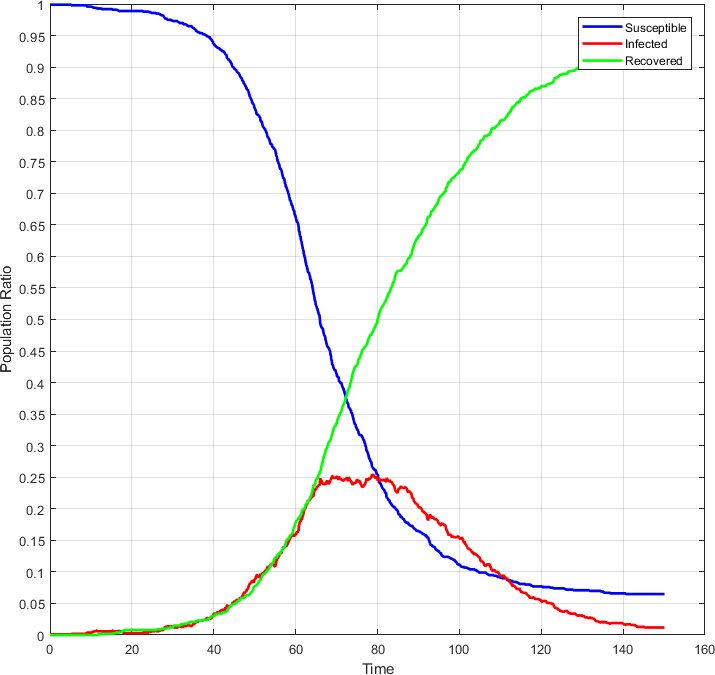
\includegraphics[width=1\textwidth, angle=0]{./fig/timedriven/SIR_Yampa/SIR_Yampa_dt01.png}
			\caption{$\Delta t = 0.1$}
			\label{fig:sir_abs_approximating_01dt_1000agents}
		\end{subfigure}
		
		&
    	
		\begin{subfigure}[b]{0.4\textwidth}
			\centering
			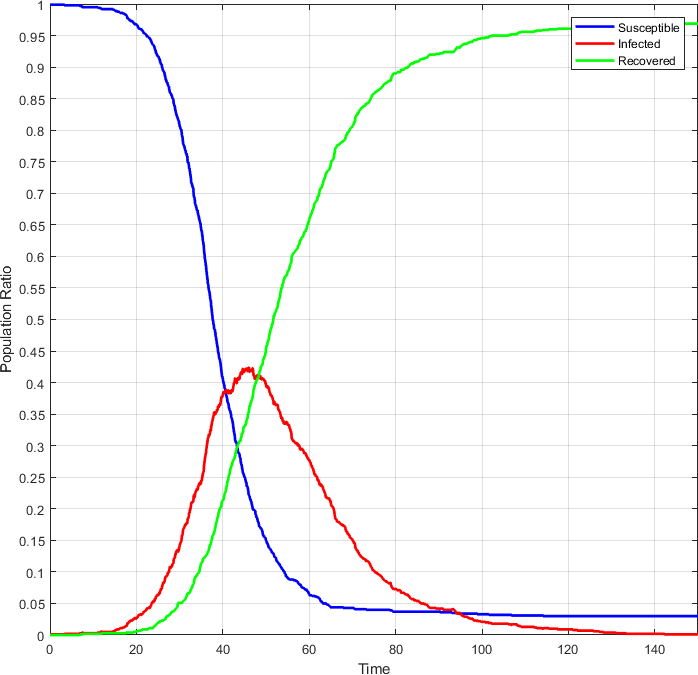
\includegraphics[width=1\textwidth, angle=0]{./fig/timedriven/SIR_Yampa/SIR_Yampa_dt001.png}
			\caption{$\Delta t = 0.01$}
			\label{fig:sir_abs_approximating_001dt_1000agents}
		\end{subfigure}
	\end{tabular}
	
	\caption{FRP simulation of agent-based SIR showing the influence of different $\Delta t$. Population size of 1,000 with contact rate $\beta = \frac{1}{5}$, infection probability $\gamma = 0.05$, illness duration $\delta = 15$ with initially 1 infected agent. Simulation run for 150 time-steps with respective $\Delta t$.} 
	\label{fig:sir_abs_dynamics_frp}
\end{center}
\end{figure}

By following the FRP approach we assume a continuous flow of time, which means that we need to select a \textit{correct} $\Delta t$, otherwise we would end up with wrong dynamics. The selection of a correct $\Delta t$ depends in our case on \textit{occasionally} in the susceptible behaviour, which randomly generates an event on average with \textit{contact rate} following the exponential distribution. To arrive at the correct dynamics, this requires us to sample \textit{occasionally}, and thus the whole system, with small enough $\Delta t$ matching the frequency of events generated by \textit{contact rate}. If we choose a too large $\Delta t$, we loose events, which will result in wrong dynamics as can be seen in Figure \ref{fig:sir_abs_approximating_01dt_1000agents}. This issue is known as under-sampling and is described in Figure \ref{fig:sampling_issue}.

\begin{figure}
\begin{center}
	\begin{tabular}{c}
		\begin{subfigure}[b]{0.5\textwidth}
			\centering
			
\includegraphics[width=1\textwidth, angle=0]{./fig/timedriven/undersampling.png}
			\caption{Under-sampling}
			\label{fig:undersampling}
		\end{subfigure}
		
		\\
		
		\begin{subfigure}[b]{0.5\textwidth}
			\centering
			
\includegraphics[width=1\textwidth, angle=0]{./fig/timedriven/supersampling.png}
			\caption{Super-sampling}
			\label{fig:supersampling}
		\end{subfigure}
	\end{tabular}
	
	\caption{A visual explanation of under-sampling and super-sampling. The black dots represent the time-steps of the simulation. The red dots represent virtual events, which occur at specific points in continuous time. In the case of under-sampling, 3 events occur in between the two time steps but \textit{occasionally} only captures the first one. By increasing the sampling frequency either through a smaller $\Delta t$ or super-sampling all 3 events can be captured.} 
	\label{fig:sampling_issue}
\end{center}
\end{figure}

For tackling this issue we have three options. The first one is to use a smaller $\Delta t$ as can be seen in \ref{fig:sir_abs_approximating_001dt_1000agents}, which results in the whole system being sampled more often, thus reducing performance. The second option is to step the simulation with $\Delta t = 1$ and in each step, instead of using \textit{occasionally}, to make a number of contacts drawn from the exponential distribution. Note that if we follow this option, we abandon the time-driven approach altogether because we don't abstract away from $\Delta t$ and violate the fundamental abstraction of FRP, which assumes that time is continuous and signal functions are running conceptually infinitely fast and infinitely often \cite{winograd-cort_wormholes:_2012}. This leaves us with the third option to implement super-sampling and apply it to \textit{occasionally}, which allows us then to run the whole simulation with $\Delta t = 1.0$ and only sample the \textit{occasionally} function with a much higher frequency.

The function \textit{embed}, which allows to run a given signal function with provided $\Delta t$, does not help here because it does not return a signal function. What we need is a signal function which takes the number of super-samples \textit{n}, the signal-function \textit{sf} to sample and returns a new signal function, which performs super-sampling on it. We provide a full implementation of such a function, which also gives an insight into how signal functions are implemented in Yampa, and how the $\Delta t$ is hidden:

\begin{HaskellCode}
import FRP.Yampa.InternalCore

-- SF is the signal-function defined for time t = 0 and returns
-- a continuation of type SF' which is the signal-function 
-- defined for t > 0: it receives an additional time-delta
-- data SF a b  = SF { sfTF :: a -> (SF' a b, b) }
-- data SF' a b = DTime -> a -> (SF' a b, b)

superSampling :: Int -> SF a b -> SF a [b]
superSampling n sf0 = SF { sfTF = tf0 }
  where
    -- no supersampling at time 0
    tf0 :: a -> (SF' a b, [b])
    tf0 a0 = (tfCont, [b0])
      where
        (sf', b0) = sfTF sf0 a0 -- running the SF
        tfCont    = superSamplingAux sf'

    superSamplingAux :: SF' a [b]
    superSamplingAux sf' = SF' tf
      where
        tf :: DTime -> a -> (SF' a b, [b])
        tf dt a = (tf', bs)
          where
            (sf'', bs) = superSampleRun n dt sf' a
            tf'        = superSamplingAux sf''

    superSampleRun :: Int -> DTime -> SF' a b -> a -> (SF' a b, [b])
    superSampleRun n dt sf a 
        | n <= 1    = superSampleMulti 1 dt sf a []
        | otherwise = (sf', reverse bs)  -- reverse due to accumulator
      where
        superDt   = dt / fromIntegral n
        (sf', bs) = superSampleMulti n superDt sf a []

    superSampleMulti :: Int -> DTime -> SF' a b -> a -> [b] -> (SF' a b, [b])
    superSampleMulti 0 _ sf _ acc  = (sf, acc)
    superSampleMulti n dt sf a acc = superSampleMulti (n-1) dt sf' a (b:acc) 
      where
        (sf', b) = sfTF' sf dt a -- running the SF'
\end{HaskellCode}

It evaluates the \textit{SF} argument for \textit{n} times, each with $\Delta t = \frac{\Delta t}{n}$ and the same input argument \textit{a} for all \textit{n} evaluations. At time 0 no super-sampling is performed and just a single output of the \textit{SF} argument is calculated. A list of \textit{b} is returned with length of \textit{n} containing the result of the \textit{n} evaluations of the \textit{SF} argument. If 0 or less super samples are requested exactly one is calculated. %We could then wrap the occasionally function which would then generate a list of events. 

\subsection{Discussion}
We can conclude that our first step already introduced most of the fundamental concepts of ABS:
\begin{itemize}
	\item Time - the simulation occurs over virtual time which is modelled explicitly, divided into \textit{fixed} $\Delta t$, where at each step all agents are executed.
	\item Agents - each agent is implemented as an individual, with the behaviour depending on its state. It is clear to see that agents behave as signals: when the system is sampled with $\Delta t = 0$ then their behaviour will stay constant and won't change because it is completely determined by the flow of time. 
	\item Feedback - the output state of the agent in the current time-step $t$ is the input state for the next time-step $t + \Delta t$.
	\item Environment - as environment we implicitly assume a fully-connected network (complete graph) where every agent 'knows' every other agent, including itself and thus can make contact with all of them.
	\item Stochasticity - it is an inherently stochastic simulation, which is indicated by the random-number generator and the usage of \textit{occasionally}, \textit{randomBoolSF} and \textit{drawRandomElemSF}.
	\item Deterministic - repeated runs with the same initial random-number generator result in same dynamics. This may not come as a surprise but in Haskell we can guarantee that property statically already at compile time because our simulation runs \textit{not} in the IO Monad. This guarantees that no external, uncontrollable sources of non-determinism can interfere with the simulation.
	\item Parallel, lock-step semantics - the simulation implements a \textit{parallel} update-strategy where in each step the agents are run isolated in parallel and don't see the actions of the others until the next step.
\end{itemize}

Using FRP in Yampa results in a clear, expressive and robust implementation. State is implicitly encoded, depending on which signal function is active. By using explicit time-semantics with \textit{occasionally} we can achieve extremely fine grained stochastics by sampling the system with small $\Delta t$: we are treating it as a truly continuous time-driven agent-based system.

A severe problem, hard to find with testing, is the fact that in the susceptible agent the same random-number generator is used in \textit{occasionally}, \textit{drawRandomElemSF} and \textit{randomBoolSF}. This means that all three stochastic functions, which should be independent from each other, are inherently correlated. This is something one wants to prevent under all circumstances in a simulation, as it can invalidate the dynamics on a very subtle level. We left this severe bug in for explanatory reasons, as it shows an example where functional programming actually encourages very subtle bugs if one is not careful. A possible but not very elegant solution would be to simply split the initial random-number generator in \textit{sirAgent} three times and pass three random-number generators to \textit{susceptibleAgent}. A much more elegant solution would be to use the \textit{Rand} Monad which, unfortunately is not possible because Yampa is not monadic.

So far we have an acceptable implementation of an agent-based SIR approach. What we are lacking at the moment is a general treatment of an environment and an elegant solution to the random number correlation. In the next step we make the transition to Monadic Stream Functions (MSFs) as introduced in Dunai \cite{perez_functional_2016}, which allows FRP within a monadic context and gives us a way for an elegant solution to the random number correlation.

\section{Second Step: Going Monadic}
A part of the library Dunai is BearRiver, a wrapper which re-implements Yampa on top of Dunai, which should allow us to easily replace Yampa with MSFs. This will enable us to run arbitrary monadic computations in a signal function, solving our problem of correlated random numbers through the use of the Random Monad.

\subsection{Identity Monad}
We start by making the transition to BearRiver by simply replacing Yampas signal function by BearRivers', which is the same but takes an additional type parameter \textit{m}, indicating the monadic context. If we replace this type-parameter with the Identity Monad, we should be able to keep the code exactly the same, because BearRiver re-implements all necessary functions we are using from Yampa. We simply re-define the agent signal function, introducing the monad stack our SIR implementation runs in:

\begin{HaskellCode}
type SIRMonad = Identity
type SIRAgent = SF SIRMonad [SIRState] SIRState
\end{HaskellCode}

\subsection{Random Monad}
Using the Identity Monad does not gain us anything but it is a first step towards a more general solution. Our next step is to replace the Identity Monad by the Random Monad, which will allow us to run the whole simulation within the Random Monad with the full features of FRP, finally solving the problem of correlated random numbers in an elegant way. We start by re-defining the SIRMonad and SIRAgent:

\begin{HaskellCode}
type SIRMonad g = Rand g
type SIRAgent g = SF (SIRMonad g) [SIRState] SIRState
\end{HaskellCode}

The question is now how to access this Random Monad functionality within the MSF context. For the function \textit{occasionally}, there exists a monadic pendant \textit{occasionallyM} which requires a MonadRandom type-class. Because we are now running within a MonadRandom instance we simply replace \textit{occasionally} with \textit{occasionallyM}. 

\begin{HaskellCode}
occasionallyM :: MonadRandom m => Time -> b -> SF m a (Event b)
-- can be used through the use of arrM and lift
randomBoolM :: RandomGen g => Double -> Rand g Bool
-- this can be used directly as a SF with the arrow notation
drawRandomElemSF :: MonadRandom m => SF m [a] a
\end{HaskellCode}

\subsection{Discussion} 
Running in the Random Monad solved the problem of correlated random numbers and elegantly guarantees us that we won't have correlated stochastics as discussed in the previous section. In the next step we introduce the concept of an explicit discrete 2D environment.

\section{Third Step: Adding an environment}
\label{sec:adding_env}
So far we have implicitly assumed a fully connected network amongst agents, where each agent can see and 'knows' every other agent. This is a valid environment and in accordance with the System Dynamics inspired implementation of the SIR model but does not show the real advantage of ABS to situate agents within arbitrary environments. Often, agents are situated within a discrete 2D environment \cite{epstein_growing_1996} which is simply a finite $N x M$ grid with either a Moore or von Neumann neighbourhood (Figure \ref{fig:abs_neighbourhoods}). Agents are either static or can move freely around with cells allowing either single or multiple occupants.

We can directly map the SIR model to a discrete 2D environment by placing the agents on a corresponding 2D grid with an unrestricted neighbourhood. The behaviour of the agents is the same but they select their interactions directly from the shared read-only environment, which will be passed to the agents as input. This allows agents to read the states of all their neighbours, which tells them if a neighbour is infected or not. To show the benefit over the System Dynamics approach  and for purposes of a more interesting approach, we restrict the neighbourhood to Moore (Figure \ref{fig:moore_neighbourhood}).

\begin{figure}
\begin{center}
	\begin{tabular}{c c}
		\begin{subfigure}[b]{0.3\textwidth}
			\centering
			
\includegraphics[width=0.5\textwidth, angle=0]{./fig/timedriven/neumann.png}
			\caption{von Neumann}
			\label{fig:neumann_neighbourhood}
		\end{subfigure}
    	&
		\begin{subfigure}[b]{0.3\textwidth}
			\centering
			
\includegraphics[width=0.5\textwidth, angle=0]{./fig/timedriven/moore.png}
			\caption{Moore}
			\label{fig:moore_neighbourhood}
		\end{subfigure}
    \end{tabular}
	\caption{Common neighbourhoods in discrete 2D environments of Agent-Based Simulation.}
	\label{fig:abs_neighbourhoods}
\end{center}
\end{figure}

We also implemented this spatial approach in Java using the well known ABS library RePast \cite{north_complex_2013}, to have a comparison with a state of the art approach and came to the same results as shown in Figure \ref{fig:sir_dunai}. This supports, that our pure functional approach can produce such results as well and compares positively to the state of the art in the ABS field.

\subsection{Implementation}
We start by defining the discrete 2D environment for which we use an indexed two dimensional array. Each cell stores the agent state of the last time-step, thus we use the \textit{SIRState} as type for our array data. Also, we re-define the agent signal function to take the structured environment \textit{SIREnv} as input instead of the list of all agents as in our previous approach. As output we keep the \textit{SIRState}, which is the state the agent is currently in. Also we run in the Random Monad as introduced before to avoid the random number correlation. 

\begin{HaskellCode}
type Disc2dCoord = (Int, Int)
type SIREnv      = Array Disc2dCoord SIRState

type SIRAgent g  = SF (Rand g) SIREnv SIRState
\end{HaskellCode}

Note that the environment is not returned as output because the agents do not directly manipulate the environment but only read from it. Again, this enforces the semantics of the \textit{parallel} update-strategy through the types where the agents can only see the previous state of the environment and see the actions of other agents reflected in the environment only in the next step.

Note that we could have chosen to use a StateT transformer with the \textit{SIREnv} as state, instead of passing it as input, with the agents then able to arbitrarily read/write, but this would have violated the semantics of our model because actions of agents would have become visible within the same time-step.

The implementation of the susceptible, infected and recovered agents are almost the same with only the neighbour querying now slightly different. 

Stepping the simulation needs a new approach because in each step we need to collect the agent outputs and update the environment for the next next step. For this we implemented a separate MSF, which receives the coordinates for every agent to be able to update the state in the environment after the agent was run. Note that we need use \textit{mapM} to run the agents because we are running now in the context of the Random Monad. This has the consequence that the agents are in fact run sequentially one after the other but because they cannot see the other agents actions nor observe changes in the shared read-only environment, it is \textit{conceptually} a \textit{parallel} update-strategy where agents run in lock-step, isolated from each other at conceptually the same time.
  
\begin{HaskellCode}
simulationStep :: RandomGen g => [(SIRAgent g, Disc2dCoord)]
               -> SIREnv -> SF (Rand g) () SIREnv
simulationStep sfsCoords env = MSF (\_ -> do
  let (sfs, coords) = unzip sfsCoords 
  -- run agents sequentially but with shared, read-only environment
  ret <- mapM (`unMSF` env) sfs
  -- construct new environment from all agent outputs for next step
  let (as, sfs') = unzip ret
      env' = foldr (\ (a, coord) envAcc -> updateCell coord a envAcc) 
               env (zip as coords)

      sfsCoords' = zip sfs' coords
      cont       = simulationStep sfsCoords' env'
  return (env', cont))
 
updateCell :: Disc2dCoord -> SIRState -> SIREnv -> SIREnv
\end{HaskellCode}

\subsection{Results}
We implemented rendering of the environments using the gloss library which allows us to cycle arbitrarily through the steps and inspect the spreading of the disease over time visually as seen in Figure \ref{fig:sir_dunai}.

\begin{figure}
\begin{center}
	\begin{tabular}{c c}
		\begin{subfigure}[b]{0.4\textwidth}
			\centering
			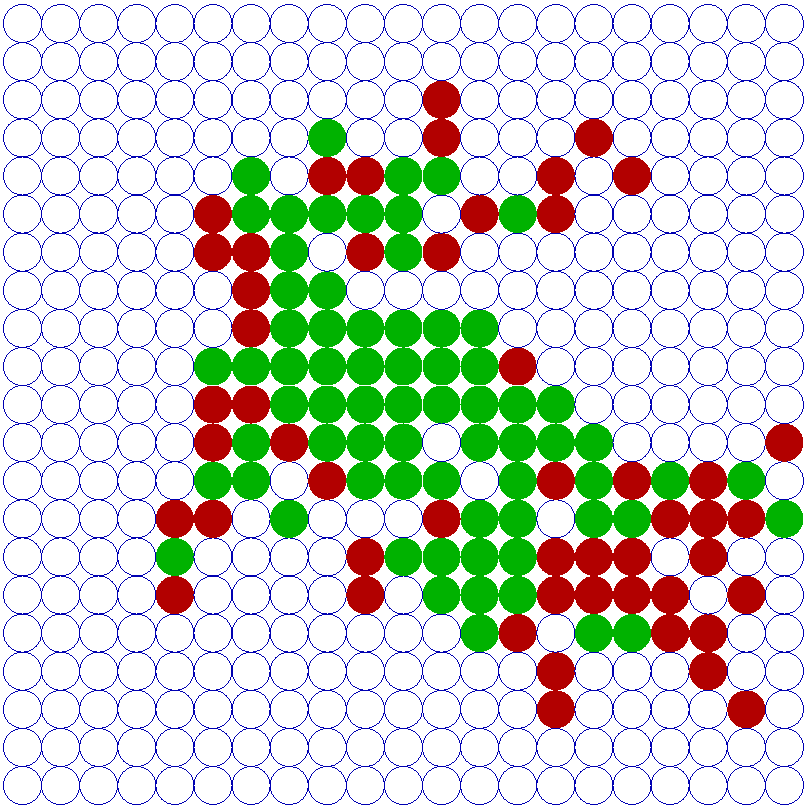
\includegraphics[width=1\textwidth, angle=0]{./fig/timedriven/SIR_Dunai/SIR_Dunai_dt001_environment.png}
			\caption{Environment at $t = 50$}
			\label{fig:sir_dunai_env}
		\end{subfigure}
    	
    	&
  
		\begin{subfigure}[b]{0.43\textwidth}
			\centering
			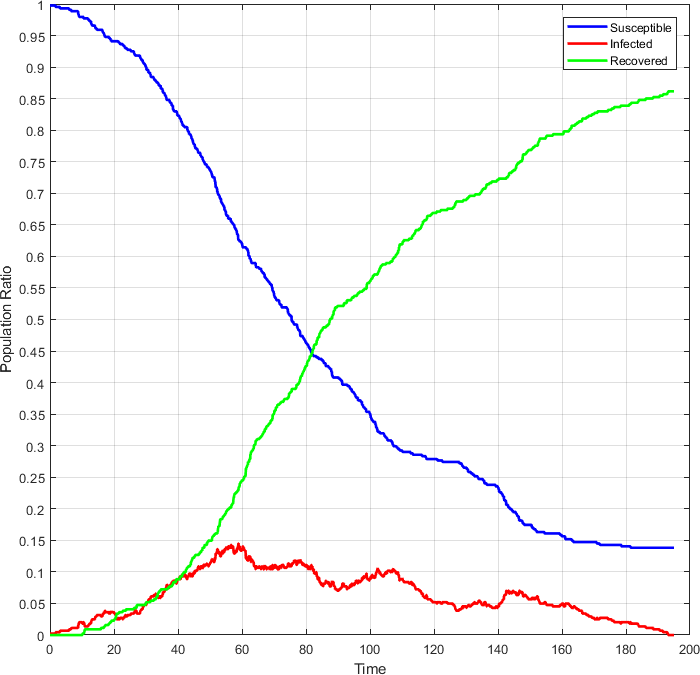
\includegraphics[width=1\textwidth, angle=0]{./fig/timedriven/SIR_Dunai/SIR_Dunai_dt001.png}
			\caption{Dynamics over time}
			\label{fig:sir_dunai_env_dynamics}
		\end{subfigure}
	\end{tabular}
	
	\caption{Simulating the agent-based SIR model on a 21x21 2D grid with Moore neighbourhood (Figure \ref{fig:moore_neighbourhood}), a single infected agent at the center and same SIR parameters as in Figure \ref{fig:sir_sd_dynamics}. Simulation run until $t = 200$ with fixed $\Delta t = 0.01$. Last infected agent recovers around $t = 194$. The susceptible agents are rendered as blue hollow circles for better contrast.}
	\label{fig:sir_dunai}
\end{center}
\end{figure}

Note that the dynamics of the spatial SIR simulation, which are seen in Figure \ref{fig:sir_dunai_env_dynamics} look quite different from the reference dynamics of Figure \ref{fig:sir_sd_dynamics}. This is due to a much more restricted neighbourhood which results in far fewer infected agents at a time and a lower number of recovered agents at the end of the epidemic, meaning that fewer agents got infected overall.

\subsection{Discussion}
By introducing a structured environment with a Moore neighbourhood, we showed the ABS ability to place the heterogeneous agents in a generic environment, which is the fundamental advantage of an agent-based approach over other simulation methodologies and allows us to simulate much more realistic scenarios.

Note, that an environment is not restricted to be a discrete 2D grid and can be anything from a continuous N-dimensional space to a complex network - one only needs to change the type of the environment and agent input and provide corresponding neighbourhood querying functions. 

\section{Discussion}
Although there are similarities to the work of \cite{botta_time_2010} (the use of messages and the problem of when to advance time in models with arbitrary number synchronised agent-interactions), we approach our agents differently. First in our approach an agent is only a single MSF and thus can not be directly queried for its internal state / its id or outgoing messages, instead of taking a list of messages, our agents take a single event/message and can produce an arbitrary number of outgoing messages together with an observable state - note that this would allow to query the agent for its id and its state as well by simply sending a corresponding message to the agents MSF and requiring the agent to implement message handling for it. Also the state of our agents is \textit{completely} localised and there is no means of accessing the state from outside the agent, they are thus "fully encapsulated agents" \cite{botta_time_2010}. Note that the authors of \cite{botta_time_2010} define their agents with a polymorphic agent-state type \textit{s}, which implies that without knowledge of the specific type of \textit{s} there would be no way of accessing the state, rendering it in fact also fully encapsulated. The problem of advancing time in our approach is solved not exactly the same but conceptually it is the same: after sending a tick message to each agent (in random order), we process all agents until they are idle: there are no more enqueued messages / events in the queue.

our eventdriven approach makes heavy use of 2 state monads, thus one might ask what the benefits are, after all we seem to fall back into stateful, imperative style programming. we agree that our approach is just one way of implementing abs in fp but we think we have come a long way thus making our approach quite valuable even if there might be other approaches like shallow EDSLs. on the other hand even our stateful programming is highly restricted to only those 2 local datatypes which makes it much more manageable than unrestricted data mutation

quote carmack (\url{http://www.gamasutra.com/view/news/169296/Indepth_Functional_programming_in_C.php}): the main difficulty as a developer in software programming is to keep track of the states a program can be in and reason about them and their Validity

TODO: report LoC and compare it with other implementations we found on the internet